\documentclass{amsart}
\usepackage{fullpage}

\usepackage[T1]{fontenc}
\usepackage[utf8]{inputenc} 
\usepackage{lmodern}
\usepackage[slovene]{babel}
\usepackage{hyperref}
\usepackage{amsmath,amssymb,amsfonts, mathtools}
\usepackage{bbm}
\usepackage{graphicx}
\graphicspath{{./images/}}

\linespread{1.2}

\newcommand{\N}{\mathbb{N}}
\newcommand{\Z}{\mathbb{Z}}
\newcommand{\Q}{\mathbb{Q}}
\newcommand{\R}{\mathbb{R}}
\newcommand{\C}{\mathbb{C}}

% ukazi za matematicna okolja
\theoremstyle{definition} % tekst napisan pokoncno
\newtheorem{definicija}{Definicija}[section]
\newtheorem{primer}[definicija]{Primer}
\newtheorem{opomba}[definicija]{Opomba}

\renewcommand\endprimer{\hfill$\diamondsuit$}


\theoremstyle{plain} % tekst napisan posevno
\newtheorem{lema}[definicija]{Lema}
\newtheorem{izrek}[definicija]{Izrek}
\newtheorem{trditev}[definicija]{Trditev}
\newtheorem{posledica}[definicija]{Posledica}

\title{Kontekstno-neodvisne gramatike za kodiranje in stiskanje podatkov}
\author{Janez Podlogar}
\date{\today}

\begin{document}

\begin{abstract}

    V delu predstavimo motivacijo in definicije, ki so potrebni za obravnavnje
    stiskanja podatkov s kontekstno-neodvisnimi gramatikami.

\end{abstract}

\maketitle

\section{Kodiranje podatkov}

Zapis informacije v neki obliki ni primeren za vsakršno rabo. Besedilo, zapisano z 
pismenkami, je neberljivo za slepe osebe, saj je komunikacijski kanal v tem primeru
vid. Prav tako pisanega besedila v pravotni obliki ni moč poslati z telegrafom. V tem
primeru je komunikacijski kanal žica in pismenke se po njej ne morejo sprehoditi. V obeh 
primerih je informacija, ki bi jo radi prenesli v neprimerni obliki. V prvem 
primeru je potrebno besedilo zapisati z Braillovo pisavo. V drugem primeru pa je 
potrebno besedil pretvoriti v električni signal. Spreminjanje zapisa sporočila
pravimo \textit{kodiranje}, sistemu pravil, po katerem se kodiranje opravi,
pa \textit{kod}. 

\begin{primer}

    \textit{Morsejeva abeceda} je kodiranje črk, števil in ločil s pomočjo zaporedja kratkih
    in dolgih signalov:

    \begin{itemize}
        \item Dolžina kratkega signala je ena enota.
        \item Dolgi signal je trikrat daljši od kratkega signala.
        \item Razmiki med signali znotraj znaka so dolžine kratkega signala.
        \item Presledki med znaki so dolgi tri kratke signale oz. en dolgi signal.
        \item Presledki med besedami so dolgi sedem kratkih signalov.
    \end{itemize}

    \begin{figure}[h]
        \centering
        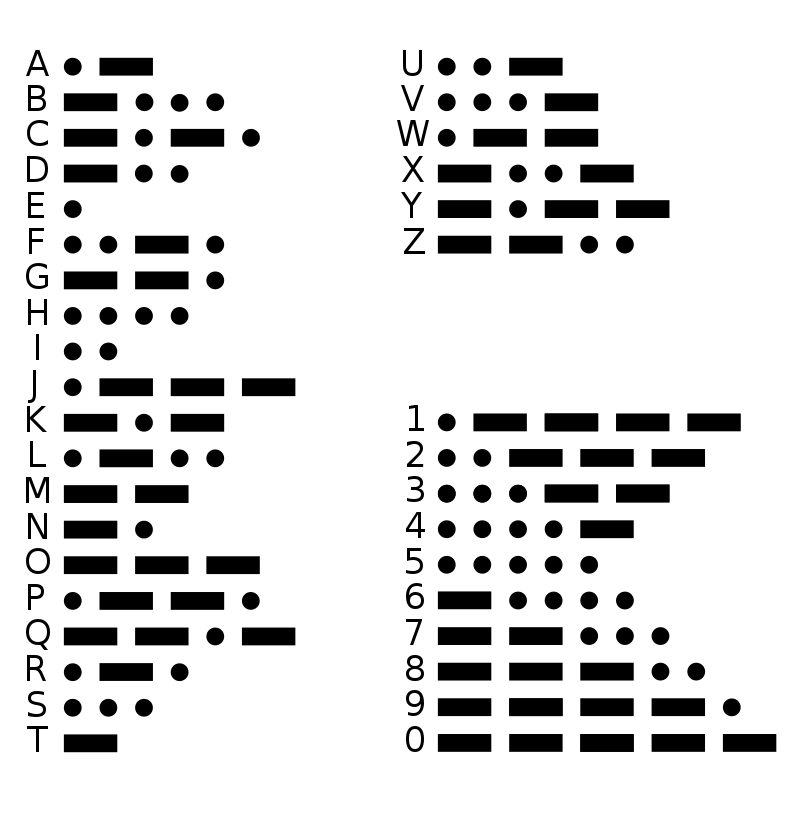
\includegraphics[width=4.3cm]{International_Morse_Code.svg.png}
        \caption{Mednarodna Morsejeva abeceda}
    \end{figure}

    Prvotni namen Morsejeve abecede je komunikacija preko telegrama, saj komunikacijski
    kanal dovoljuje le električne signale in tišino med njimi. Kodiranje črk je takšno,
    da imajo črke z višjo frekvenco (v angleškem jeziku) krajši zapis, s tem se dolžina
     kodiranega sporočila skrajša in posledično tudi čas prenosa.

\end{primer}

\begin{definicija}

    \textit{Abeceda} je neprazna množica $ \Sigma $. \textit{Množica vseh končnih besed na 
    abecedi} $ \Sigma $ je

    \begin{equation*}
        \Sigma^* = \{\, a_1 a_2 a_3 \cdots a_n \mid n \in \N \land \forall i: a_i \in \Sigma \,\} \cup \{ \varepsilon \}, 
    \end{equation*}

    kjer $ \varepsilon $ prazna beseda. Jezik na abecedi $ \Sigma $ je poljubna podmnožica množice vseh 
    besed $ \Sigma^* $.

\end{definicija}

\begin{opomba}
    
    V splošnem ima lahko abeceda poljubno kardinalnost, v diplomski nalogi se bomo srečali le z končnimi abecedami.

\end{opomba}

\begin{primer}
    
    Naj bo $ \Sigma = \{\, a,b,c \,\} $ abeceda, potem je

    \begin{align*} 
        ab \in \Sigma^* \\
        ccc \in \Sigma^* \\
        cababcccababcccab \in \Sigma^*
    \end{align*}

\end{primer}

\section{Stiskanje podatkov}

Namenov kodiranja je tudi doseči čim večjo ekonomičnost zapisa. Želimo, da bi bilo naše sporočilo čim
 krajše. Kodiranje, ki skrajša zapis podatkov, imenujemo \textit{stiskanje podatkov}.

\begin{primer}\label{p1}
    
    Ponovno za abecedo vzemimo $ \Sigma = \{\, a,b,c \,\} $ in poglejmo besedo

    \begin{equation*}
        \mathbf{x} = cababcccababcccab
    \end{equation*}

    Opazimo, da se nam v besedi $ \mathbf{x} $ večkrat ponovita vzorca $ ab $ in $ ccc $. Zato uvedemo
    novi spremenljivki $ A_1 = ab $ in $ A_2 = ccc $. Sedaj lahko zapišemo $ \mathbf{x} $ kot

    \begin{equation*}
        \mathbf{x} = cA_1A_1A_2A_1A_1A_2A_1
    \end{equation*}

    Ponovno se nam pojavi vzorec, tokrat $ A_1A_1A_2 $. Uvedemo novo spremeljivko $ A_3 = A_1A_1A_2 $
    in zapišemo $ \mathbf{x} $ kot

    \begin{equation*}
        \mathbf{x} = cA_3A_3A_1
    \end{equation*}
    
    Prvotno besedilo smo z novimi spremeljivkami uspešno skrajšali. Kot bomo videli kmalu, smo
    pretvorili besedo $ \mathbf{x} $ v kontekstno neodvisno gramatiko $ \mathbf{G_x} $ z 
    produkcijskimi pravili

    \begin{align*}
        & A_0 \, \rightarrow \, cA_3A_3A_1, \\
        & A_1 \, \rightarrow \, ab, \\
        & A_2 \, \rightarrow \, ccc, \\
        & A_3 \, \rightarrow \, A_1A_1A_2.
    \end{align*}

\end{primer}

\section{Kontekstno-neodvisne gramatike}



\begin{definicija}

    \textit{Formalna gramatika} $ G $ so pravila, ki nam iz abecede $ \Sigma $ tvorijo jezik
    $ \mathbf{L}(G) $

\end{definicija}

\begin{definicija}

    \textit{Kontektsno-neodvisna gramatika} je četverica $ G = (\, V, \Sigma, P, S \,) $, kjer je
    $ V $ končna množica \textit{spremenljivk}, $ \Sigma $ množica \textit{končnih simbolov} tako,
    da $ \Sigma \cap V = \emptyset $, $ P \subseteq V \times (\, V \cup \Sigma \,)^* $ množica 
    \textit{produkcijskih pravil}, $ S \in V $ \textit{začetna spremenljivka}.

\end{definicija}

% Besede so sestavljenje samo iz elementov abecede. Nizi so sestavljeni tako iz
% končnih terminalov kot iz spremeljivk. Morda bi milo smiselno označevati ene z
% grškimi črkami in druge z latinico.

\begin{definicija}
    
    Naj bo $ G = (\, V, \Sigma, P, S \,) $ kontekstno-neodvisna gramatika. Naj bodo $ \mathbf{x} $,
    $ \mathbf{y} $, $ \mathbf{z} \in (\, V \cup \Sigma \,)^* $ nizi spremenljivk in končnih simbolov,
    $ A \in V $ spremenljivka ter naj bo $ ( A, \mathbf{y} ) \in P $ produkcijsko pravilo,
    označimo ga z $ A \rightarrow \mathbf{y} $. Pravimo, da $ \mathbf{x}A\mathbf{z} $ 
    \textit{pridela} $ \mathbf{x}\mathbf{y}\mathbf{z} $, pišemo
    $ \mathbf{x}A\mathbf{z} \, \Rightarrow \, \mathbf{x}\mathbf{y}\mathbf{z} $. Pravimo, da
    $ \mathbf{x} $ \textit{porodi} $ \mathbf{y} $, če je $ \mathbf{x} = \mathbf{y} $ ali če
    za $ k \geq 0 $ obstaja zaporedje nizov $ \mathbf{x_1}, \mathbf{x_2}, \ldots \mathbf{x_n}
    \in (\, V \cup \Sigma \,)^* $ tako, da 

    \begin{equation*}
        \mathbf{x} \Rightarrow \mathbf{x} \Rightarrow \mathbf{x_1} \Rightarrow \ldots \Rightarrow \mathbf{x_n}
        \Rightarrow \mathbf{y}
    \end{equation*}
    in pišemo $ \mathbf{x} \xRightarrow{*} \mathbf{y} $.

\end{definicija}

\begin{posledica}

    Jezik kontekstno neodvisne gramatike $ G $ je 

    \begin{equation*}
        \mathbf{L}(G) = \{\, \mathbf{u} \in \Sigma^* \mid S \xRightarrow{*} \mathbf{u} \,\}.
    \end{equation*}

\end{posledica}

\begin{opomba}
    
    Ime kontekstno-neodvisna gramatika izvira iz oblike produkcijskih pravil. Na levi strani produkcijskega
    pravila mora vedno stati samo spremenljika. Torej, ne sme vsebovati pravila oblike

    \begin{equation*}
        A\mathbf{u} \rightarrow \mathbf{v},
    \end{equation*}
    kjer je $ A \in V $ in $ \mathbf{u} $, $ \mathbf{v} \in \Sigma $, saj bo pravilo pridelalo 
    $ \mathbf{v} $ saj samo, če se niz končana $ \mathbf{u} $. Torej je odvisno od predhodnega
    konteksta.

\end{opomba}

\begin{primer}
    
    Formalizirajmo gramatiko iz Primera~\refeq{p1}, ki smo jo generirali iz $ \mathbf{x} $
    Označimo jo z $ \mathbf{G_x} = (\, V, \Sigma, P, S \,) $, kjer je 

    \begin{align*}
        & V = \{\, A_0, A_1, A_2, A_3 \,\}, \\
        & \Sigma = \{\, a, b, c \,\}, \\
        & P = \{\, A_0 \, \rightarrow \, cA_3A_3A_1, A_1 \, \rightarrow \,
          ab, A_2 \, \rightarrow \, ccc, A_3 \, \rightarrow \, A_1A_1A_2 \,\}, \\
        & S = A_0.
    \end{align*}
    Vidimo, da $ \mathbf{G_x} $ ustreza naši definiciji kontekstno-neodvisne gramatike
    in res kodira $ \mathbf{x} $, saj je 

    \begin{equation*}
        \mathbf{L}(\mathbf{G_x}) = \mathbf{x} 
    \end{equation*}

\end{primer}

\end{document} 